\documentclass[11pt]{article}
\usepackage{graphicx}
\usepackage{listings}
\usepackage{caption}

%title page
%-----------------------------------------------------------


\author{Zola Mahlaza}
\title{\textbf{Functional Programming} \\ Black jack using scheme}
\date{\today}

%-----------------------------------------------------------

\begin{document}
	\begin{figure}
	\centering
	\includegraphics[scale=0.5]{uct_logo.jpeg}
	\end{figure}
	\maketitle
	
	%--------------------------------------
	%	Beginning the actual document
	%--------------------------------------
	\section{Introduction}
	Functional programming
	\section{Results}
	There are tasks which have been automated. Listing \ref{python} is the source code that creates a 100 hands used to to test strategies. It is used to generate hands in general.
	
	\subsection{Best Hand}
	This function computes the best hand. There is only choice when there
	is an ace in the given hand. This function makes the ace count as 1 or
	11 depending on which is the 'best hand'. The test runs of this function are provided are shown in listing \ref{besthand}
	
	\subsection{Stop at n}
	This function is a strategy whose logic lies in picking a point
	to stop taking a hit. Listing \ref{stopatn} shows the test results of 
	this function. When the value of n is small, the probability of requesting a hit is small and as n increases, so does the probability. Figure \ref{graph1} is an illustration of this.
	\section{Appendix}
	
		\subsection{Data}
		
		%python script
		\begin{lstlisting}[caption=python script that generates hands randomly, label=python]
		
from random import randint
suit = {1:'c', 2:'d', 3:'s', 4:'h'}
numbers ={
		1:'A',
		2:'2',
		3:'3',
		4:'4',
		5:'5',
		6:'6',
		7:'7',
		8:'8',
		9:'9',
		10:'K',
		11:'Q',
		12:'J'
	}
def main():
	print(gen_file(2))
#method for making a list of lists
def gen_file(n):
	defin = '(define myfile \n\'('
	for i in range(n):
		defin += '('+gen_hand()+' '+gen_card()+')\n'
	defin += '))'
	return defin

#method for generating a hand
def gen_hand():
	size = randint(2,4)
	hand = '('
	for i in range(size):
		hand += gen_card() +' '
	hand += ')'
	return hand
#Method for generating a random card
def gen_card():
	return '('+numbers[gen_num(1,12)]+' '+suit[gen_num(1,4)]+')'
#Method for generating a number between Min and Max(inclusive)
def gen_num(Min, Max):
	return randint(Min,Max)
if __name__=='__main__':
	main()
		\end{lstlisting}



	%%%%%%%%%%%%%%%%%%%%%%%%%%%%%%%%%%%%%%%%%%%%%%%%%
	%												%
	%	The followind is the result for a few tests %
	%   of best-hand. The hands given are random	%
	%												%
	%%%%%%%%%%%%%%%%%%%%%%%%%%%%%%%%%%%%%%%%%%%%%%%%%
	\begin{lstlisting}[caption=results of best hand test runs, label=besthand]

(best-hand '((J h) (Q h) (7 d) ))
27
(best-hand '((A d) (A d) (3 s) ))
15
(best-hand '((5 c) (7 h) ))
12
(best-hand '((4 h) (6 s) (7 h) ))
17
(best-hand '((5 d) (9 c) ))
14
(best-hand '((Q c) (6 h) (6 c) (6 d) ))
28
(best-hand '((7 h) (J s) (Q s) ))
27
(best-hand '((2 h) (A c) (A h) ))
14
(best-hand '((A h) (7 c) (8 s) ))
16
(best-hand '((J c) (9 c) (J c) (J s) ))
39
(best-hand '((2 h) (2 c) ))
4
(best-hand '((Q h) (A d) ))
21
(best-hand '((Q h) (7 d) ))
17
(best-hand '((Q s) (8 c) ))
18
(best-hand '((3 c) (2 s) (4 d) ))
9
(best-hand '((2 s) (4 h) (J c) (2 h) ))
18
	\end{lstlisting}
	
	\begin{lstlisting}[caption=Results of testing stop-at-n with 1000 hands and different values of n, label=stopatn]

Here, 1 and 0 represent true and false respectively.
 
n = 10	
0,0,0,0,0,0,0,0,0,0,0,0,0,0,0,0,0,0,0,0,0,0,0,0,0,0,0,1,0,0,0,0,0,0,0,0,0,0,0,0,0,0,0,0,0,0,1,0,0,0,0,0,0,0,1,0,0,0,0,0,0,0,0,0,0,0,0,0,0,0,1,0,0,0,0,0,0,0,0,0,0,0,0,0,0,0,0,0,0,0,0,0,0,0,0,0,0,0,0,0,0,0,0,0,0,0,0,0,0,0,0,0,0,0,0,0,0,0,0,0,0,0,0,0,0,0,0,1,0,0,0,0,0,0,0,0,0,0,0,0,0,1,0,0,0,0,0,0,0,0,0,0,0,0,0,0,0,0,0,0,0,0,0,0,0,0,0,0,0,0,0,0,0,0,0,0,0,0,0,0,1,0,0,0,0,0,0,0,0,0,0,0,0,0,0,0,0,0,0,0,0,0,0,0,0,0,0,0,0,0,0,0,0,0,0,0,0,0,0,0,0,0,0,0,0,0,0,0,0,0,0,0,0,0,0,0,1,0,1,0,0,0,0,0,0,0,0,0,0,0,0,0,0,0,0,0,0,0,0,0,0,0,0,0,0,0,0,0,0,0,0,0,0,0,0,1,0,0,1,0,0,0,0,0,0,0,0,0,0,0,0,0,0,0,0,0,0,0,0,0,0,0,0,0,0,0,0,0,0,0,0,1,0,0,0,0,0,0,0,0,0,0,0,0,0,0,0,0,0,0,0,0,0,0,0,0,0,0,0,0,0,0,0,0,0,0,0,0,0,1,0,0,0,0,0,0,0,0,0,0,0,0,0,0,0,0,0,0,0,0,0,0,0,0,1,0,0,0,0,0,0,0,0,0,0,0,0,0,0,0,0,0,0,0,0,0,0,0,1,0,0,0,0,0,0,0,0,0,0,0,0,0,1,0,1,0,0,0,0,0,0,0,0,0,0,0,0,0,0,0,0,0,0,0,0,0,0,0,0,0,0,0,0,0,0,0,0,0,0,0,0,0,0,0,0,0,0,0,0,0,0,0,0,0,0,0,0,0,0,0,0,0,0,0,0,0,0,0,0,0,0,0,0,0,0,0,0,0,0,0,0,0,0,0,0,1,0,0,1,0,0,0,0,0,1,0,0,0,0,0,0,0,0,0,0,0,0,0,0,0,0,0,0,0,0,0,0,0,0,0,0,0,0,1,0,0,0,0,0,0,0,0,0,0,0,0,0,0,0,0,0,0,0,0,0,1,0,0,0,0,0,0,0,0,0,0,0,0,0,0,0,0,0,0,0,0,0,0,0,0,0,0,0,0,0,0,0,0,0,0,0,0,0,0,0,0,0,0,0,0,0,0,0,0,0,0,0,0,0,0,0,0,0,0,0,0,0,0,0,0,0,0,0,0,0,0,0,0,0,0,0,0,1,0,0,0,0,0,0,0,0,0,0,0,1,0,0,0,1,0,0,0,0,0,0,0,0,0,0,0,0,1,0,0,0,0,0,0,0,0,0,0,0,0,0,0,0,0,0,0,0,0,0,0,0,0,0,0,0,0,1,1,0,0,0,0,1,1,0,0,0,0,0,0,0,0,0,0,0,0,0,0,0,0,0,0,0,0,0,1,0,0,0,0,0,0,0,0,0,0,0,0,0,0,0,0,0,0,0,0,0,0,0,0,0,0,0,0,0,0,0,0,0,0,0,0,0,0,0,0,0,0,0,0,0,0,0,0,0,0,0,0,0,0,0,0,0,0,0,0,0,0,0,0,0,0,0,0,0,0,0,0,0,0,0,0,0,0,0,0,0,0,0,0,0,0,0,0,0,0,0,0,0,0,0,0,0,0,0,0,0,0,1,0,0,0,0,0,0,0,0,0,0,1,0,0,0,0,0,0,0,1,0,0,1,0,0,0,0,0,0,0,0,0,0,0,0,1,0,0,0,0,0,0,0,0,0,0,0,0,0,0,0,0,0,0,0,0,0,0,0,0,0,0,0,0,0,0,0,0,0,0,0,0,0,0,0,0,0,0,0,0,0,0,0,0,0,0,0,0,0,0,0,0,0,0,0,0,0,0,0,0,0,0,0,0,0,0,0,0,0,0,0,0,0,0,0,0,0,0,0,0,0,0,0,0,0,0,0,0,0,0,0,0,0,0,0,0,0,0,0,0,0,0,0,0,0,0,0,0,0,0,0,0,1,0,0,0,0,0,0,0,0,0,0,0,0,0,0,0,0,0,0,0,0,0,0,0,0,0

n = 15
1,1,0,1,0,0,0,0,0,0,0,0,0,1,0,0,0,0,0,0,0,0,0,0,1,0,1,1,0,1,0,0,0,0,1,0,0,0,0,0,1,0,0,0,0,0,1,1,0,0,1,0,1,0,1,0,0,0,0,0,0,0,0,0,1,0,0,1,0,1,1,0,0,0,0,1,0,1,0,0,0,0,1,0,0,0,0,0,0,0,0,0,0,0,1,0,0,1,0,0,0,1,0,0,0,0,0,0,0,1,0,0,0,0,0,1,0,0,0,0,0,0,0,0,0,0,0,1,0,0,0,0,0,0,0,1,1,0,0,0,0,1,0,0,0,1,0,0,0,0,0,0,0,1,1,0,1,1,0,1,1,0,0,0,0,0,0,0,0,0,0,0,1,0,1,0,0,0,0,0,1,1,0,1,0,1,0,0,0,0,0,0,1,0,0,0,1,0,0,0,0,0,1,0,0,0,0,0,0,0,0,0,0,0,0,0,0,1,0,0,0,0,0,1,0,0,1,0,0,0,0,0,0,0,0,1,1,0,1,0,0,1,1,0,0,0,0,0,1,1,0,0,0,0,1,0,0,0,0,0,1,0,0,0,0,0,1,0,0,0,0,0,0,0,0,1,1,0,1,0,0,0,1,0,0,0,1,0,0,1,0,0,0,0,0,0,1,1,0,0,1,0,0,1,0,0,1,0,0,0,0,1,1,0,0,0,1,0,1,0,0,0,0,0,0,0,0,0,0,0,0,1,0,0,1,0,0,0,0,1,1,0,0,0,1,0,0,0,0,1,1,0,0,0,0,0,0,0,1,0,0,0,1,0,1,0,0,0,0,1,1,0,0,0,1,0,0,0,0,1,0,0,0,0,0,0,1,0,0,0,0,0,0,1,1,0,0,0,1,0,0,0,0,0,0,0,0,1,0,0,1,0,1,0,1,1,0,1,0,0,0,1,0,0,0,1,0,1,0,0,0,0,0,0,1,0,1,0,0,0,0,1,0,0,0,0,0,0,0,1,0,0,0,0,0,0,0,0,0,1,0,0,0,0,0,0,0,0,1,1,0,0,0,0,0,0,1,0,1,1,1,0,0,0,0,0,0,0,0,1,0,0,1,0,0,1,0,0,1,1,1,0,0,0,1,0,0,0,1,0,0,0,0,0,1,0,0,0,1,0,0,0,0,0,0,1,0,1,0,0,0,1,0,1,0,0,0,1,0,0,0,0,0,0,0,0,1,1,1,0,0,0,0,0,1,1,0,0,0,0,0,0,0,0,0,0,0,0,0,0,0,0,0,0,0,0,0,1,0,0,0,0,0,1,1,1,0,0,0,0,1,0,0,0,0,0,0,0,0,0,0,0,0,1,0,0,0,0,0,0,0,0,0,0,0,0,1,0,0,0,0,0,0,1,1,0,0,0,0,0,0,0,1,0,0,0,0,0,1,0,1,0,0,1,1,1,0,0,1,0,1,0,0,0,0,0,0,0,0,0,0,1,0,0,0,0,0,0,0,0,1,0,0,1,1,1,0,0,0,0,0,0,0,0,1,1,0,0,0,0,1,1,0,1,0,1,1,1,1,0,0,1,0,0,0,0,1,0,0,0,0,0,0,0,0,0,1,0,0,1,0,0,0,0,0,0,0,0,1,0,0,0,0,0,0,0,0,0,0,0,0,0,0,0,1,1,1,0,0,0,0,0,0,0,0,0,0,0,0,0,1,0,0,1,1,0,0,1,0,0,0,1,1,0,0,0,0,1,0,0,0,0,0,1,0,1,0,0,0,0,1,0,0,0,0,1,0,0,0,0,0,0,1,1,0,0,1,0,0,0,0,0,0,0,0,0,0,0,0,1,0,0,1,0,0,0,0,1,0,0,0,1,1,1,1,0,1,0,0,1,1,1,1,1,1,0,0,0,0,0,0,1,1,0,0,0,0,1,1,0,0,0,1,0,0,0,1,0,0,0,0,0,0,0,0,0,0,0,0,1,0,0,0,0,1,0,0,0,1,0,0,0,1,0,0,0,0,0,0,0,0,0,0,0,0,0,0,1,0,0,0,0,0,0,0,0,1,0,0,0,0,0,1,0,1,0,0,0,0,0,0,0,0,0,0,0,0,1,0,0,0,0,0,0,1,0,0,0,0,0,1,0,0,0,0,0,0,0,0,1,0,0,0,0,0,1,0,0,0,1,0,0,0,0,1,0,0,0,0,0,0,0,0,1,0,0,0,0,0,0,1,0,0,1,0,1,0,0,0,0

n = 20
1,1,0,1,1,0,0,0,0,1,0,1,0,1,0,0,0,1,0,0,0,0,0,1,1,0,1,1,0,1,0,0,1,0,1,1,0,0,0,0,1,0,0,1,1,0,1,1,0,0,1,0,1,1,1,0,0,1,1,1,1,0,1,1,1,0,1,1,1,1,1,1,0,0,0,1,1,1,0,0,0,1,1,1,0,1,0,1,0,0,1,1,0,0,1,1,1,1,0,0,0,1,1,0,0,0,0,1,0,1,1,0,0,1,0,1,1,0,0,0,0,0,1,0,0,0,1,1,0,0,1,0,0,0,0,1,1,1,0,0,0,1,0,0,0,1,0,0,1,1,0,1,0,1,1,1,1,1,0,1,1,0,0,0,1,1,0,0,0,1,1,1,1,1,1,0,0,1,1,1,1,1,0,1,1,1,0,0,0,1,1,1,1,0,0,0,1,0,0,1,0,0,1,1,1,1,0,0,1,0,0,0,1,1,0,1,0,1,0,0,0,1,0,1,1,0,1,0,0,0,0,0,0,0,0,1,1,0,1,0,1,1,1,0,1,0,0,0,1,1,0,1,1,0,1,0,0,1,0,1,1,1,1,0,0,0,1,0,1,0,1,1,0,0,0,1,1,0,1,0,0,1,1,1,0,1,1,1,0,1,1,0,0,0,0,0,1,1,1,1,1,0,0,1,0,0,1,1,0,0,0,1,1,1,0,1,1,1,1,0,0,1,0,0,1,1,0,0,0,0,0,1,0,1,1,0,0,0,0,1,1,0,0,0,1,1,0,1,1,1,1,1,1,0,0,1,0,1,1,1,0,1,1,1,1,1,1,0,0,1,1,0,0,1,1,0,0,1,1,1,1,0,1,1,1,0,1,0,1,0,0,1,0,1,1,1,1,1,1,1,0,1,0,0,0,1,0,1,0,0,1,0,1,0,1,1,0,1,1,1,0,1,0,1,0,1,0,1,0,0,1,1,0,0,1,0,1,0,0,0,0,1,0,1,0,1,0,1,0,1,0,0,0,0,1,0,0,1,1,1,0,0,1,1,1,0,0,0,1,1,0,0,0,0,1,1,1,0,1,1,1,0,1,0,1,1,1,1,0,1,1,0,1,0,1,1,0,1,1,1,1,1,0,0,1,0,0,1,1,1,0,0,0,1,1,1,0,0,1,0,0,0,0,0,1,1,1,1,1,1,1,1,1,1,0,0,1,1,0,0,1,1,0,1,0,0,1,1,1,1,1,1,1,0,1,1,0,1,1,0,0,1,1,1,1,0,0,0,0,0,1,0,0,0,0,1,0,1,0,0,1,0,1,1,1,1,1,1,1,1,1,1,0,1,0,1,1,0,0,0,1,0,1,1,0,0,1,1,1,0,0,1,0,0,1,0,1,0,1,0,0,0,0,1,1,0,1,0,0,1,1,0,1,1,1,0,0,1,1,1,1,0,0,1,1,1,0,0,1,0,1,0,0,0,0,0,1,0,0,1,0,1,0,0,1,0,0,0,1,0,1,0,0,1,1,1,1,0,0,0,0,1,0,1,1,1,1,0,0,0,1,1,1,1,0,1,1,1,1,0,0,1,0,1,0,0,1,0,0,0,0,1,1,0,1,0,1,0,1,1,0,0,1,0,0,1,1,0,1,1,0,1,0,1,0,1,0,0,1,0,1,1,0,1,1,1,1,1,0,0,0,0,0,0,0,0,0,0,1,0,1,0,0,1,1,0,1,1,0,1,1,1,1,0,0,1,1,1,0,0,0,0,0,1,0,1,0,0,1,1,1,0,1,0,1,1,0,0,0,0,0,1,1,1,1,0,1,0,0,1,1,1,0,0,0,0,1,0,0,1,0,0,1,1,1,0,0,1,1,1,1,1,1,1,1,0,1,1,0,1,1,1,1,1,1,0,1,0,1,1,1,1,1,1,0,0,1,1,1,0,0,0,1,0,0,0,1,0,1,0,0,1,1,0,1,0,1,1,1,1,0,1,0,0,1,0,0,1,1,1,1,1,1,0,1,0,1,0,1,0,1,1,1,1,0,1,1,1,1,0,1,0,0,1,0,0,1,0,0,1,0,0,1,1,1,1,0,0,0,1,0,0,0,0,0,1,1,1,0,0,0,1,0,0,1,1,0,0,0,1,1,1,0,1,1,1,1,1,0,1,0,0,0,0,0,1,0,0,1,1,1,1,0,1,1,0,0,1,0,1,0,1,0,1,0,1,0,1,1,1,1,1,0,1,1,1,0,0,0,0
	
	\end{lstlisting}
	
	
	\subsection{Figures}
		
			\begin{figure}[h]
				\centering
				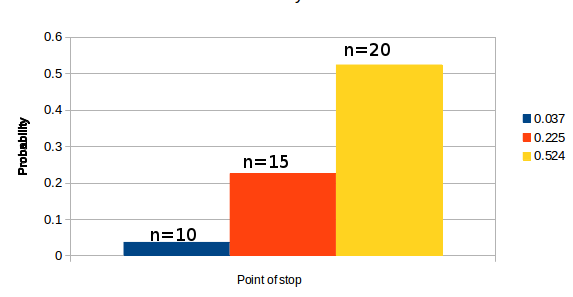
\includegraphics[scale=1]{stop-at.png}
				\caption{Probability of requesting hit}
				\label{graph1}
			\end{figure}
			
\end{document}